\chapter{WordPressBench System}
\label{chapter:chapter4}


\section{System Architecture}
\label{sub-sec:system-architecture}

WordPressBench has a master-slave architecture, with a Master defined by the Controller which creates the work-pool with tasks according to the user's settings. The tasks are then executed by the slaves, the Workload Generators. The slaves generate HTTP requests to the Web servers running WordPress. The WordPress server is the unmodified version downloaded from the official WordPress website[]. Figure 4.1 pictures the system with all the components and relations between them. Each component will be described in detail in the following sections.

  \begin{figure}[htb]
    \begin{center}
    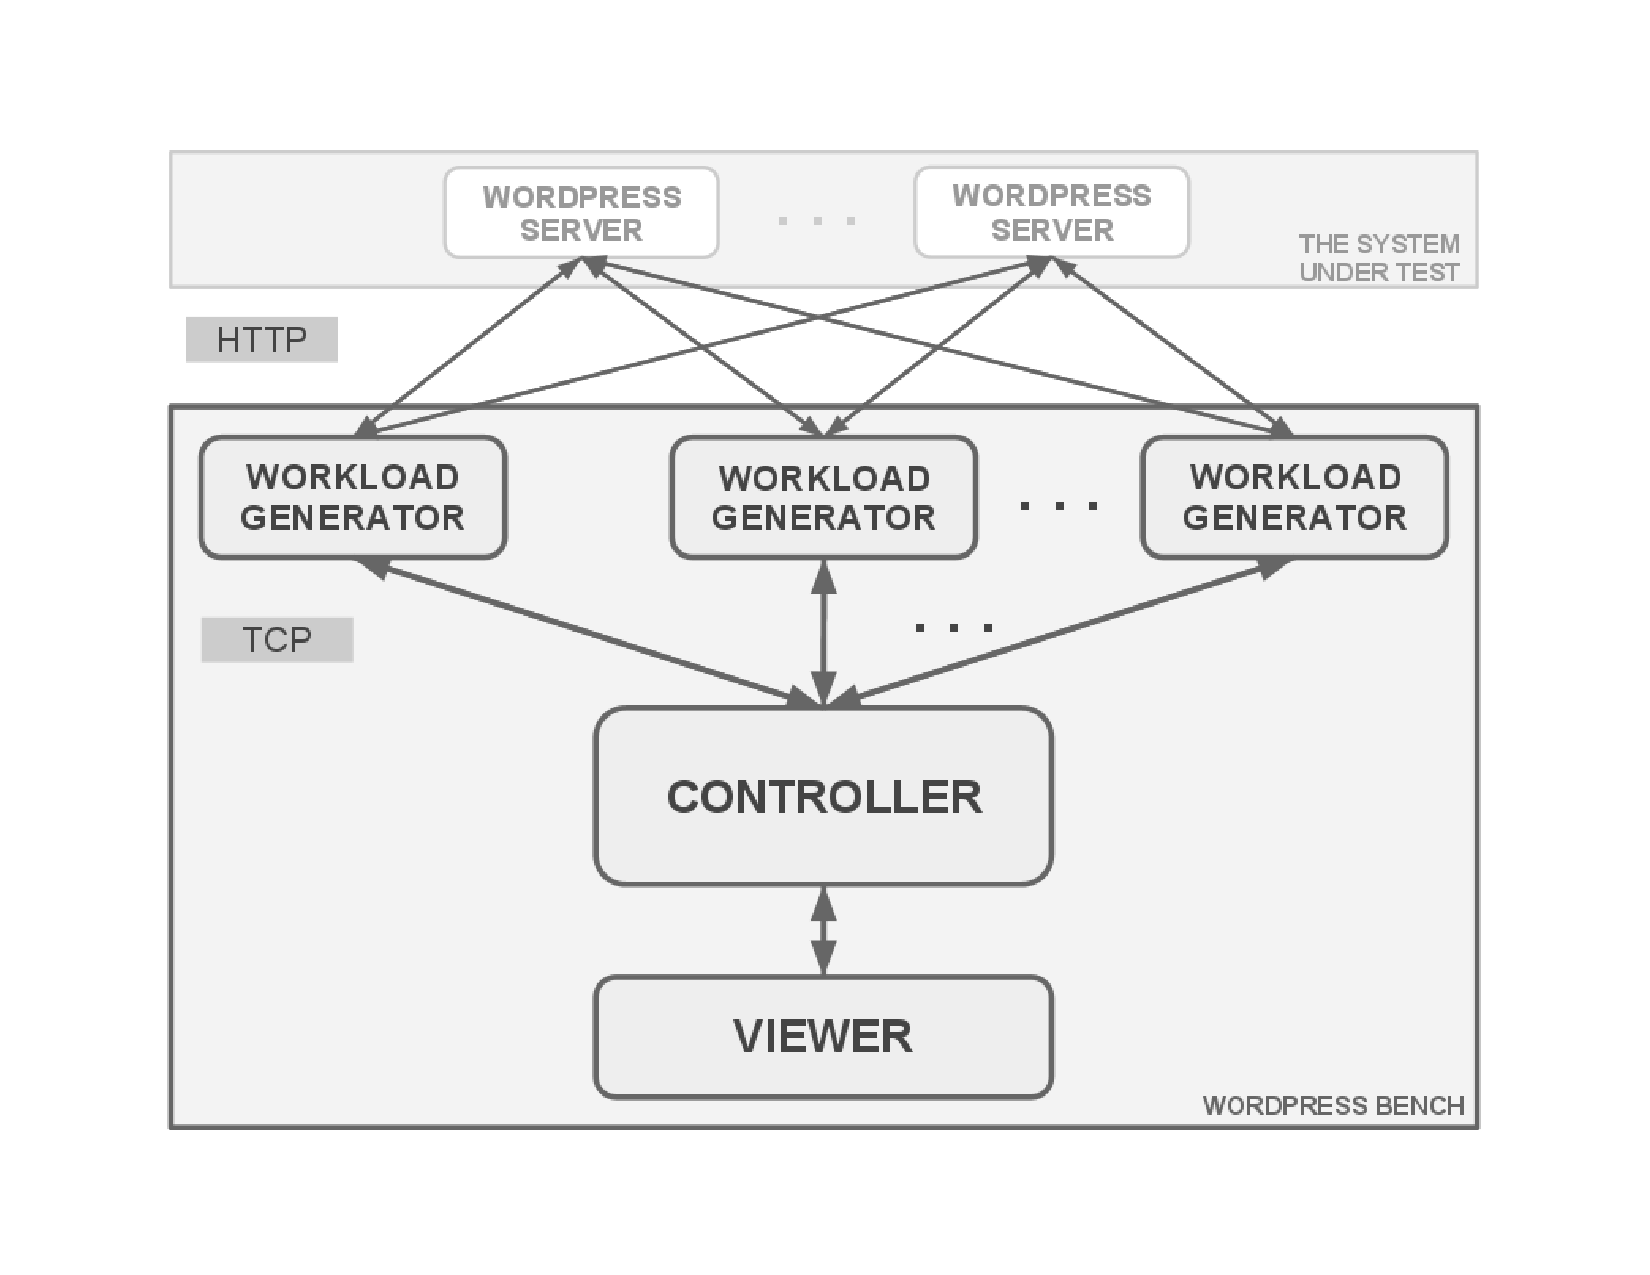
\includegraphics[trim=2.5cm 2.5cm 2.5cm 2.5cm, clip=true, scale=0.65]{src/img/WordPressBench.pdf}
    \caption{System Design}
    \end{center}
  \end{figure}

%\fig[scale=0.6]{src/img/WordPressBench.pdf}{img:system-design}{System Design}

\section{Components}
\label{sec:components}

\subsection{WordPress Web Servers}
\label{sub-sec:wordpress-web-servers}

The WordPress Web Server use Apache servers and use a MySQL database. It also requires to have PHP installed on the machine. We used WordPress version 3.2 available at the development time. It allows users to read blog-posts, pages and comments. This can be done by searching by keyword, by author, by date, by category, by viewing recent posts, or simply by browsing each single blog-post. Anonymous users are allowed to post comments by providing their e-mail address. Their information remains in browser's cache through cookies, until the information is overwritten.

Additional write operations are allowed only for registered users. After logging in, they have access to extended edit functionalities, like adding comments to pages and blog-posts as registered users, or adding pages, blog-posts and blog-post categories. Users with 'Administrator' rights are allowed to create new users, or to clear the data from the database, operation performed in the initiation stage of the development. TO CONTINUE

\subsection{Workload Generator}
\label{sub-sec:workload-generator}

The Workload Generator is a component running on slaves machines. It basically contains a Markov matrix with all the possible states and the probabilities to make a transition to another state. 

There are three transition matrices, one for anonymous user, one for logged-out user, and another for anonymous user. This is mainly because the registered user has access to additional states and the flow of actions could be totally different from an anonymous user. The read-only user has the most restrictive operations.

The transition matrix describes the users' navigational pattern, by specifying how users navigate through the website, the functions they are allowed to use in a certain state and how often, and the frequency of transitions from one state to another. Users interact with the WordPress Website through sessions, which are sequences of consecutive requests to bring different pages from the WordPress Website. After each request, a transition is made from the current state to another state. The next state is chosen from the transition matrix which indicates for each state which are the next possible transitions. The matrix columns indicate the current state, and the matrix lines are the states which could follow. A zero in the matrix means that there is no transition from current state to the state indicated by the line. A non-zero value in the matrix represents the probability to make a transition to the state indicated by the line. So when choosing the next state, only a non-zero value will be chosen. For building the transition matrix we chose bigger probabilities for widely used functionalities, like reading a blog-post or posting a comment. Image 4.2 depicts the transition table for a registered user who can log-in and perform additional write operations.

%   \begin{figure}[htb]
%     \begin{center}
%     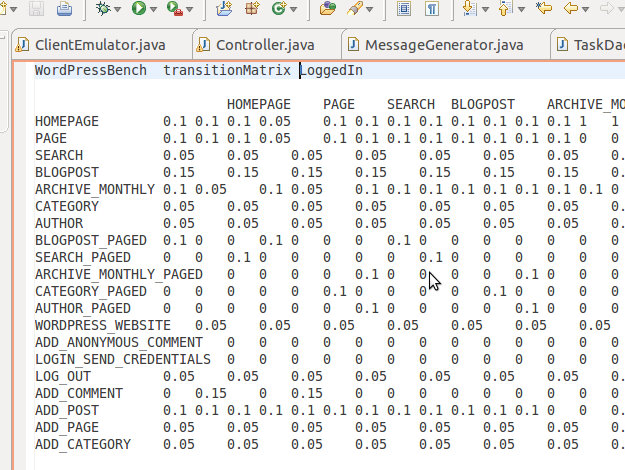
\includegraphics[scale=0.8]{src/img/transitionTable.jpg}
%     \caption{Transition matrix for a Logged-in user}
%     \end{center}
%   \end{figure}

  \begin{figure}[t]
    \centering %trim=l b r t
    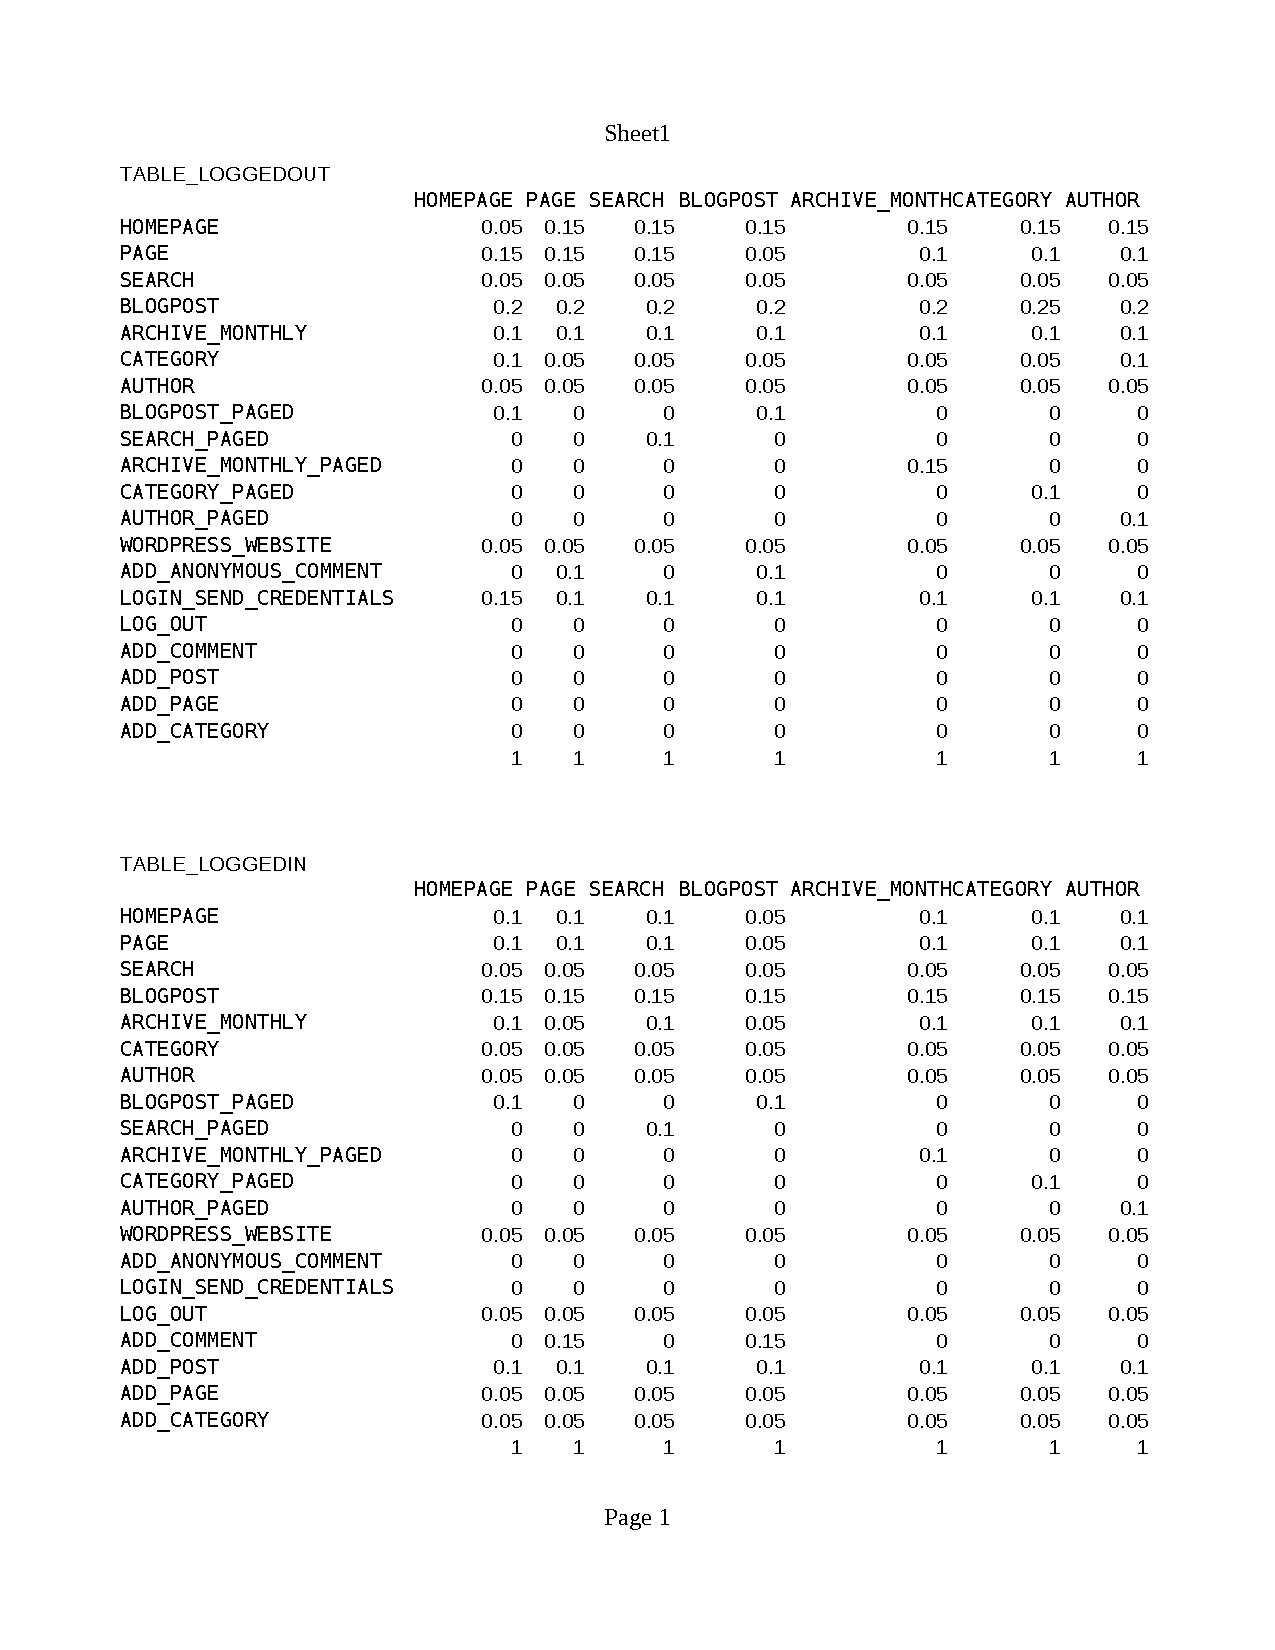
\includegraphics[trim=2cm 14cm 2cm 3.2cm, clip=true, scale=0.85]{src/img/transitionTable.pdf}
    \caption{Transition matrix for a Logged-in user}
  \end{figure}

The HTTP requests require URLs which specify what page should be brought back. Additional information is oftenly needed, especially for users who are logged-in, so information is either encoded in POST variables, or in cookies. The information which is requested by the WordPress servers includes user information, text for publishing, IDs, options, nonces (random number issued in previous HTML content received from WordPress server), passwords and usernames. Some of this information is generated by the Workload Generator, but the IDs or nonces are gathered from the previous HTTP page just received from the WordPress server. Cookies also need to be send back to the server, exactely as they have been received. They are used to maintain the logged-in user session, and they are reset as soon as the user loggs-out. If the request is succesfull, and the correct page is sent back, the session makes a transition to the desired state. To simulate users more realistically and knowing that real users spend a different amount of time between requests, each emulated user has a random "think time" of at least 7 seconds between requests.

In case a user loggs in, the session is maintained through cookies, which need to be sent back to the Web server at each request until the user logs out. There are states which get data from HTTP POST variables, not only from GET variables encoded in URLs. In this case, the slave needs to get the keywords, IDs, from the previous page, and send it along with other random data generated on the fly, and needed by the Web server. 

While running, the Workload Generator gathers statistics about the responses time. Statistics like response time, number of errors, number of attempts before getting the response, or other such information is stored for each user along with a timestamp, and aggregated into log files which are sent to the Master at the end of the simulation.

\subsection{Controller}
\label{sub-sec:controller}

The Controller is the main command component. It has control over the Workload Generators and sends commands to them through TCP messages. The Controller can send five types of messages:
\begin{itemize}
 \item start simulation
 \item stop simulation
 \item create users
 \item add users
 \item get logfile.
\end{itemize}

For starting the simulation it also indicates the username range to be used by each Workload Generator, along with the read-write ratio. The command for creating more users has the effect of registering a certain amount of users to the WordPress server(s). This command is generally followed by either the simulation start, or adding more users. The latter command is send during a simulation, when new user sessions are initiated. The log file command simply receives the log files with statistics from each Workload Generator, which are then aggregated and processed to be displayed on the user interface. The username range, or the number of users to be added or started is computed for each Workload Generator, so they won't overlap.

\subsection{Graphic Interface}
\label{sub-sec:graphic-interface}


\section{Workflow}
\label{sec:workflow}

- the connection between components\\
- how does it work as a whole


\section{Tools and Technologies}
\label{sec:tools-and-technologies}

- the technologies used: WordPress, Apache, MySQL, Java, HTTP protocol, TCP connections